
\documentclass[journal]{IEEEtran}

% *** GRAPHICS RELATED PACKAGES ***
%

  %\usepackage[pdftex]{graphicx}
  \usepackage{graphicx}
  \usepackage{amsmath}
  \usepackage{hyperref}
  \usepackage{media9}
  % declare the path(s) where your graphic files are
 \graphicspath{{./images/}}
  % and their extensions so you won't have to specify these with
  % every instance of \includegraphics
   \DeclareGraphicsExtensions{.pdf,.jpeg,.png,.jpg}
\usepackage[export]{adjustbox}
\usepackage{float}

\usepackage[section]{placeins}

% correct bad hyphenation here
\usepackage{fixltx2e}
 \usepackage{cite} 
\usepackage{url}

\usepackage{epstopdf}

\epstopdfDeclareGraphicsRule{.gif}{png}{.png}{convert gif:#1 png:\OutputFile}
\AppendGraphicsExtensions{.gif}

\setcounter{totalnumber}{5}
\setcounter{topnumber}{5}
\setcounter{bottomnumber}{5}
\renewcommand{\topfraction}{1}
\renewcommand{\bottomfraction}{1}

\begin{document}

%
% paper title
% can use linebreaks \\ within to get better formatting as desired
% Do not put math or special symbols in the title.
\title{A Look at Virtual Reality Implementations}
%
%
% author names and IEEE memberships
% note positions of commas and nonbreaking spaces ( ~ ) LaTeX will not break
% a structure at a ~ so this keeps an author's name from being broken across
% two lines.
% use \thanks{} to gain access to the first footnote area
% a separate \thanks must be used for each paragraph as LaTeX2e's \thanks
% was not built to handle multiple paragraphs
%

\author{Gautam Baghel\\Richard (Alex) Showalter-Bucher}

	\maketitle

% Add a link target to the TOC itself
\addtocontents{toc}{\protect\hypertarget{toc}{}}
\addtocontents{toc}{\setcounter{tocdepth}{1}}


\newpage
\tableofcontents
\newpage
%\listoffigures
%\listoftables

\section{Introduction}
In our project within this course, we explored implementing VR into three open source games: Super Mario HD (a Unity remake of the first stage of Super Mario 64), FreeSpace 2 and Quake. As an extension to that work, we sought out to explore how our virtual reality (VR) implementations, as well as several other game implementations, differ in experience and presence. In this paper we discuss the different implementations of VR games using the following concepts:


\begin{itemize}
	\item Locomotion
	\item Controls
	\item Interaction
	\item Visualization
	\item Social Aspects
	\item Comfort
	\item Immersion
\end{itemize}

 
By the end of the paper, you should have a better understanding of different approaches to those concepts in VR games and software. 

\section{Concept Definitions}
Before we can discuss games in terms of the concepts mentioned in the introduction, we need to give our definitions of each concept. The following are our definitions. 


\subsection{Locomotion}
Locomotion will be a discussion of the methodology to be able to move about the 3D world. In many traditional games, movement is based on inputs from a trackpad, d-pad, or joystick.  In virtual reality there is a spectrum of different methodologies of movement. As an example, some of the more common VR locomotion types are trackpad/joystick, teleportation, and room scale movement.

\subsection{Controls}
Controls will be a discussion of how the player gives inputs for the game. This will discuss the type of controls used such as motion tracked or gamepad controllers as well as how each button is mapped for the controllers. 

\subsection{Interaction}
Interaction will be a discussions of how the player can directly interact with the world. This is an interesting topic due to the closer mapping of natural tendencies from true reality to the virtual world such as picking up a book on a table or hitting an object with your hands. Below is a 5 level system which we can rate the interactiveness. \newline\newline
\textit{\textbf{Interaction Level}}
   \begin{enumerate}
   	\item None
   	\item A Little
   	\item Some
   	\item Mostly
   	\item Complete
   \end{enumerate}
   
\subsection{Visualization}
Visualization  will discuss the render quality and art style of the of these games. Virtual reality demands high frame rates (90 frames per second for the HTC Vive or Oculus Rift) and the ability to push two rendered scenes to each eye in the head mounted display (HMD). This gives the developers a more constrained space to implement their games  visualization. Some common art styles in VR are simplistic, cartoony, or realistic (photogrammetry). 

\subsection{Social Aspects}
A great misnomer about virtual reality is that it is an isolating experience as you are blinding yourself from the world when you put on the HMD. In contrary, VR can be more social than traditional gaming due to the fact that it can remotely place you in the same space with other people. When we discuss social aspects, we will be discussing in what ways each game allows you to socialize with other players.


\subsection{Comfort}
A common discussion topic about VR is comfort of the player during the experience. To address this topic, we will discuss how nauseating or unnatural a game's experience makes you feel. We will quantify this concept as follows: \newline\newline
\textit{\textbf{Comfort Level (Nausea)}}
\begin{enumerate}
	\item Unplayable
	\item Major
	\item Significant
	\item Minor
	\item None
\end{enumerate}

\noindent \textit{\textbf{Natural Comfort Level}}
\begin{enumerate}
	\item Completely Unnatural
	\item Mostly Unnatural
	\item Somewhat Natural 
	\item Mostly Natural
	\item Completely Natural
\end{enumerate}

\subsection{Immersion}
One key goal in virtual reality is to create a feeling of complete immersion within the virtual environment. For each game, we will discuss the level of immersion we experienced during it.  This is a very subjective matter; we will attempt to describe the aspects which we believe increased or reduced the level of immersion we experienced. 
We will quantify this concept as follows: \newline\newline
\textit{\textbf{Immersion Level}}
\begin{enumerate}
	\item None
	\item A Little
	\item Some
	\item Mostly
	\item Complete
\end{enumerate}



\section{Virtual Reality System}

For our system we chose to use the HTC Vive\cite{htc_vive}. This system consists of two base stations,a head mounted display(HMD), and two motion controllers (Figure \ref{htc_vive}).


\begin{figure}[H]

	\noindent
	\centering{\hspace{0 ex} 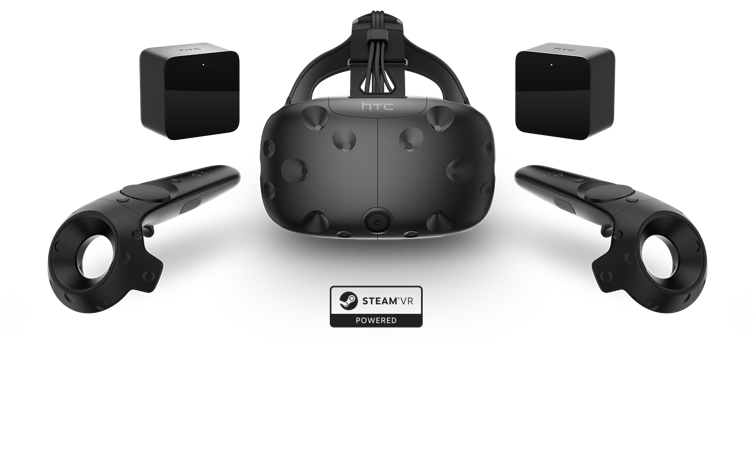
\includegraphics[width=4in]{htc_vive_headset.png}}
	\caption{Image of HTC Vive controllers, head-mounted-display, and base stations.\cite{htc_vive_system_image}}\label{htc_vive}
\end{figure}


The base stations are laser-based reference points used to remove biases inherent to the Inertial Measurement Unit (IMU) tracking and provides up to millimeter precision track errors. This, in turn, provides one-to-one correspondence to movements of the HMD and controllers in the real world. The tracking is even accurate enough to juggle the controllers while in the virtual world \cite{juggline_htc_vive_controllers}. 

The HMD consists of two 90 Hz 1080x1200 OLED screens, two Fresnel lenses, and a 110$^{\circ}$  horizontal field of view\cite{htc_vive_system_specs}.  Additionally the HMD has a build in microphone and a pass-through camera which enables you to see the room while wearing the headset. 

Both controllers are wand shape and are designed to be used in either your left or right hand (Fig. \ref{ViveControllerButtons}). They contain five buttons: trigger, system, menu, grip, and trackpad. There is also integrated haptic feedback in each controller to help simulating different experiences in the virtual world. 

The link-box provides power to the HMD and acts like a break-away box for the HDMI and USB cables that run to the headset. 



\begin{figure}[H]
	
	\noindent
	\centering{\hspace{-8 ex} 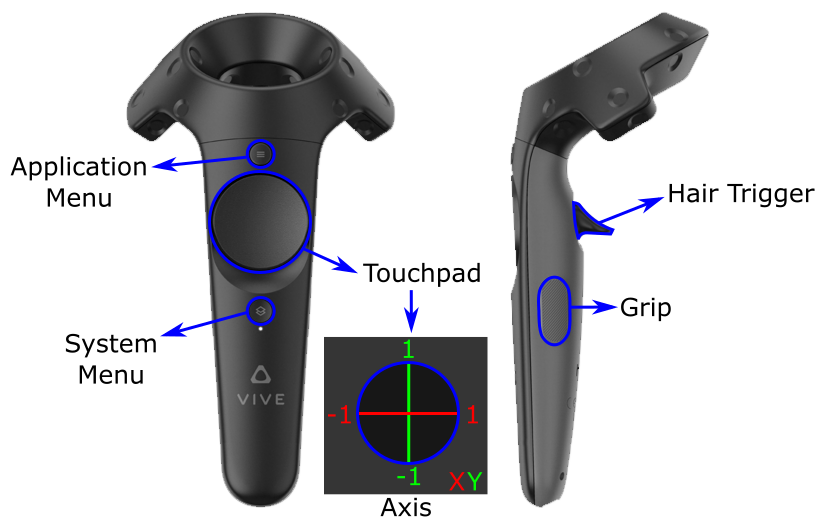
\includegraphics[width=3in]{ViveControllerButtons.png}}
	\caption{Diagram of HTC Vive controller buttons.\cite{htc_vive_controller_buttons}}\label{ViveControllerButtons}
\end{figure}


\section{Overview of Games}
In addition to the three games we've integrated virtual reality into, we have identified eight games which have some differences in their approach to virtual reality software. These games are listed in Table \ref{GAME_LIST} along with respective summaries of each concept. 



We discuss each one of these games in detail in the subsequent sections. We have also included included videos for each game that contains a discussion of the concepts along with some game play.  


 

\section{Lucky$'$s Tale}

Lucky's Tale is a free game that was released for the Oculus Rift in April 2016. Since the Oculus Rift did not support motion controllers at the time, this game exclusively uses a gamepad for it's controls. Figure \ref{LuckysTale_Gameplay} has a video discussing the different aspects of this game. 

\begin{figure}[h]
	\noindent
	\centering{\hspace{-8 ex}
	\includemedia[
	width=1.1\linewidth,height=0.61875\linewidth,
	activate=pageopen,
	flashvars={
		modestbranding=1 % no YT logo in control bar
		&autohide=1 % controlbar autohide
		&showinfo=0 % no title and other info before start
		&rel=0 % no related videos after end
	}]{}{http://www.youtube.com/v/nDbdVvUGopQ}
		\caption{Lucky's Tale Gameplay and Discussion}
		\label{LuckysTale_Gameplay}}
\end{figure}



\subsection{Locomotion}
The locomotion in Lucky's Tale is handle by the joystick on the gamepad. The movement is similar to many other popular platformers such as Crash Bandicoot or Super Mario 64. You can move the character left, right, up, and down. You can also jump to get around obstacles in the game, and you have some ability to be able to climb at specific locations. 

We should also mention that your VR headset is the camera in the game. You can move your head around in 3D space and the camera will move in the same fashion. 

\subsection{Controls}
The Oculus Rift was shipped with an Xbox One controller and since this game was developed exclusively for the Oculus Rift, the controls were designed around that. Figure gives you an example of the buttons on the Xbox One controller for reference.
\begin{figure}[H]
	
	\noindent
	\centering{\hspace{0 ex} 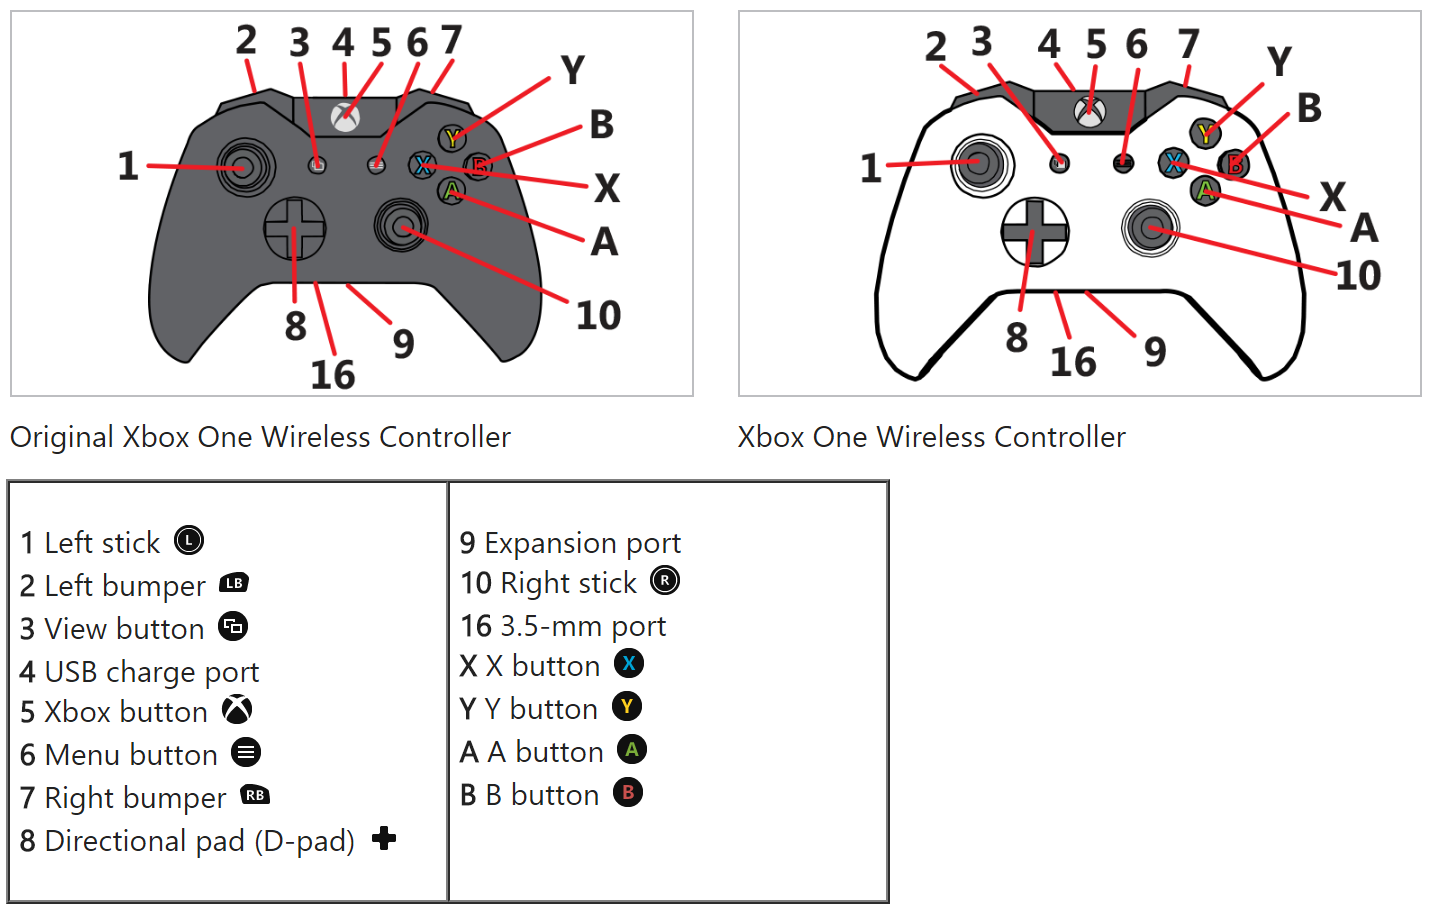
\includegraphics[width=4in]{xbox_controller.png}}
	\caption{Image of Xbox One controller.  stations.\cite{xbox_one_controller_buttons}}\label{xbox_one_controller}
\end{figure}

The controls in this game are as follows: 

\begin{itemize}
	\item The \textbf{left joystick} moves the character around
	\item The \textbf{start} button brings up the menu/pauses
	\item The \textbf{select} button centers the screen
	\item The \textbf{X} and \textbf{Y} buttons Tailswipe
	\item The \textbf{A} and \textbf{B} buttons Jump
	\item The \textbf{Left or Right Bumper} does a Belly Flop while jumping
\end{itemize}

\subsection{Interaction}
The interaction is just that of a standard platformer such as Super Mario 64. You can jump on enemies, pickup items and carry them, and break boxes. 
We would classify this as having \textbf{a little} bit of interaction. 

\subsection{Visualization}
Visually it is quite bright and cartoony. It definitely has a feel of some of the classic Nintendo 64 Platformers such as Super Mario 64 or Banjo-Kazooie but with updated graphics. 

\subsection{Social Aspects}
This game was designed to be a single player game and therefore has no social aspects integrated in it's design.


\begin{table*}[!t]
	\caption{Summary of Games}
	\label{GAME_LIST}
	\hspace{-10ex}
	\begin{tabular}{|l|l|l|l|l|l|l|l|}
		\hline
		\textbf{Name} & \textbf{LOCOMOTION} & \textbf{CONTROLS} & \textbf{INTERACTION} & \textbf{VISUALIZATION} & \textbf{SOCIAL} & 	\textbf{COMFORT} & \textbf{IMMERSION}\\
		\hline
		\hline
		Lucky's Tale\cite{luckys_tale_game} & Joystick & Gamepad & Jumping on Enemies & Cartoony & None & Naus. Minor & Mostly &		
		&          &         & Rating: A little   &          &      & Nat. Mostly &        &\hline
		
		Google Earth\cite{google_earth_game} & Flying & Motion Controller & Move Sun         & Toy Model Town & None & Naus. Minor & Mostly &
		&        &                   & Rating: A little &                &      & Nat. Mostly &        &\hline
		
		Destinations\cite{destinations_game}  & Room Scale    & Motion Controller &              & Realistic      & Hangout   & Naus. None    & Mostly &
		& Teleportation &                   & Rating: Some & Infinite Types & Mini-games& Nat. Complete &        &\hline
		
		Climbey\cite{climbey_game}  & Room Scale    & Motion Controller & Climbing on Walls & Simple & Climbing & Naus. Sig.    & Some &
		& Swinging Arms &                   & Rating: A little  & Bland  &          & Nat. Somewhat &      &\hline
		
		TheWaveVR\cite{thewavevr_game}  & Roomscale     & Motion Controller & Make Music and Trip & Psychedelic & Rave       & Naus. None    & Complete &
		& Teleportation &                   & Rating: Mostly      & Dark        & Group Trip & Nat. Complete &          &\hline
		
		Rec Room\cite{rec_room_game}  &  Room Scale   & Motion Controller & Pickup Some Objects& Cartoony & Mini-games & Naus. None    & Mostly &
		& Teleportation &                   & Mostly             & Simple    & Hang-Out  & Nat. Complete &         &\hline
		
		Rick and Morty:                             & Room Scale     & Motion Controllers & Pickup all items  & Cartoony & None & Naus. None   & Complete &
		Virtual Rick-ality\cite{rickandmorty_game}  & Preset Portals &                    &Rating: Completely & Bright   &      & Nat. Complete &          &\hline
		
		Minecraft\cite{vive_craft_game}  & Room Scale    & Motion Controllers & Collect and Craft  & Blocky & Craft   & Naus. Major & Mostly &
		(Vivecraft)                      & Teleportation &                    & Rating: Completely & 8-bit  & Explore & Nat. Mostly &        &\hline
		
		Super Mario HD\cite{super_mario_hd_game}  & Arrow Keys  & Keyboard/Mouse & Jumping on Enemies & Cartoony        & None & Naus. Minor   & A little &
		& Joystick    & Gamepad        & Rating: A little   & HD and Lighting &      & Nat. Somewhat &          &\hline
		
		FreeSpace 2\cite{freespace2_game}  & Arrow Keys & Keyboard/Mouse & Shoot Enemies        & Space & Skirmish  & Naus. Unplayable& A little&
		&            &                & Rating: A little     & Dark  & (Broken)  & Unnat. Mostly   &         &\hline
		
		Quake\cite{quake_game} & Trackpad            & Motion Controller & Shooting/Items   & Dark Palette   & Death Match & Naus. Sig.    & Mostly&
		Ver. A                 & Controller Pointing &                   & Rating: A little & Old-School FPS & (Broken)    & Nat. Somewhat &       &\hline
		
		Quake\cite{quake_game}  & Trackpad     & Motion Controller & Shooting/Items   & Dark Palette    & Death Match & Naus. Minor & Mostly&
		Ver. B                  & HMD Pointing &                   & Rating: A little & Old-School FPS  & (Broken)    & Nat. Mostly &       &\hline
		
	\end{tabular}
	
\end{table*}

\subsection{Comfort}
Overall, we found the game to be fairly comfortable. The virtual reality integration feels \textbf{mostly natural} due to the fact that you head is tracked one-to-one. It only made us feel \textbf{minor nausea}, though this may get worse with more game play time because the camera does also follow the character. 





\subsection{Immersion}

 Surprisingly this game was \textbf{mostly immersive}. It lacks complete room scale movement and you feel like a giant due to your camera perspective which does take away from the immersion. But while playing the game, we could see getting a bit lost in the world.  

\section{Google Earth VR}

This is software developed by Google which brings all of the geo-spatial information of Google Earth into virtual reality. They have not only the 2D maps of the globe, but for some locations they have 3D models. Figure \ref{GoogleEarth_Gameplay} has a video discussing the different aspects of this game. 

\begin{figure}[h]
	\centering
	\centering{\hspace{0 ex}
	\includemedia[
	width=1.1\linewidth,height=0.61875\linewidth,
	activate=pageopen,
	flashvars={
		modestbranding=1 % no YT logo in control bar
		&autohide=1 % controlbar autohide
		&showinfo=0 % no title and other info before start
		&rel=0 % no related videos after end
	}
	]{}{http://www.youtube.com/v/DNmqNiEfGEE}
		\caption{Google Earth VR Gameplay and Discussion}
		\label{GoogleEarth_Gameplay}}
\end{figure}

\subsection{Locomotion}
The main mode of locomotion in the game is flying. You achieve this by using the right-hand trackpad's button. You can also move based on selecting a new location on the globe on the left controller or in the menu. Lastly, you can move by holding in the trigger in you right-hand which allows you to drag yourself relative to where the controller was pointing when you pressed the trigger.
\subsection{Controls}
This software uses the motion controllers and the controls are as follows: 

\begin{itemize}
	\item The \textbf{Right-hand Grip} button  rotates the world
	\item The \textbf{Right-hand Menu} button brings up the menu where you can select places to go to
	\item The \textbf{Left-hand Menu} button saves current location
	\item The \textbf{Right-hand Trigger} lets you drag the world when held down. It also lets you select items in menus. 
	\item The \textbf{Left-hand Trackpad} button lets you change the Earth's tilt
	\item The \textbf{Right-hand Trackpad} lets you fly
\end{itemize}

\subsection{Interaction}
There is not much to interact with within this software. In fact, the only interaction we could find was the ability to change the time of the day by moving the sun in the sky. We rate this as having \textbf{a little} bit of interaction. 
\subsection{Visualization}
At times, the visualization is stunning and realistic since it is based on photos and data collected in the real world. The software lets you travel from space down to street level of anywhere in the world. Many, but not most, locations have 3D reconstructed buildings, cars and trees. This adds to the realism of the environment. 
\subsection{Social Aspects}
This software was designed as a single user experience. There is no integrated social aspects within the software. 
\subsection{Comfort}
The software has built-in options to improve comfort such as turning off street-level viewing as well as having a vignette to reduce your field of view when flying. With the comfort settings on, we found this game to have only \textbf{minor nausea} and it feels \textbf{mostly natural}. 
\subsection{Immersion}
This software can be extremely immerse if you are in a location with 3D reconstructed data along with being far enough away from the 3D models to not notice the artifacts from the reconstruction. Generally speaking though, it does not feel like you are truly in that location. Overall, we rate this software as being \textbf{mostly immersive}.


\section{Destinations}
Destinations is a game that enables you to experience real and fictional environments by yourself or with another person. Many of the environments within the game are 3D reconstructions of actual locations using photogrammetry. Besides exploring, this game has added in several objectives such as cache finding to help encourage users to go to different locations. Additionally they have added some mini-games to play with other users online. Figure \ref{Destinations_Gameplay} has a video discussing the different aspects of this game. 
 
\begin{figure}[h]
	\centering
	\centering{\hspace{0 ex}
	\includemedia[
	width=1.1\linewidth,height=0.61875\linewidth,
	activate=pageopen,
	flashvars={
		modestbranding=1 % no YT logo in control bar
		&autohide=1 % controlbar autohide
		&showinfo=0 % no title and other info before start
		&rel=0 % no related videos after end
	}
	]{}{http://www.youtube.com/v/3rOHPnmI5N0}
		\caption{Destinations Gameplay and Discussion}
		\label{Destinations_Gameplay}}
\end{figure}

\subsection{Locomotion}
This game's locomotion consists of both teleportation (blink) and room scale movement. Many areas of the game are open to the user to teleport or walk around. There are some locations where you are restricted to teleporting to discrete spots such as mountains, or lily pads. 
 
\subsection{Controls}
This game uses the motion controllers and the controls are as follows: 

\begin{itemize}
		\item The \textbf{Trackpad} button let's you use teleportation
		\item The \textbf{Menu} button brings up the menu where you can select different locations, items to bring into the world, customizations to your character. You can also invite other users to join your location in the menu.  
		\item Both \textbf{Grip} buttons held down resize items in your hand
		\item The \textbf{Trigger} select or pickup items. If the item has secondary functionality, you can also access that by clicking the trigger again when the item is in your hand.  


\end{itemize}
\subsection{Interaction}
Originally this game did not have much in terms of interaction. You were limited to visiting locations and reading signs. They did end up adding in props, tools, and wearables that you could collect. The props can be taken out and resized, the tools can do things such as help you find a geo-cache or shoot lasers, and the wearables can be used to dress up your avatar. Overall this game has \textbf{some} level of interaction.
\subsection{Visualization}
Like mentioned before, many of the environments within the game are 3D reconstructions of actual locations using photogrammetry. Those locations look realistic, but they do have artifacts from the reconstruction that makes it a bit off. Generally speaking, since much of the content is user generated the visualization varies drastic between the different environments. 
\subsection{Social Aspects}
This game allows you to join environments with others and walk around the same space together. It includes the ability to customize avatars, invite other players to your room, or join public spaces. They also have mini-games built into the software such as Skee ball. 
\subsection{Comfort}
Since this game uses teleportation and room-scale movement, it is a very comfortable game to play for hours. We have found no discomfort or unnaturalness in the game play. We found that the game was \textbf{completely natural} and that it had \textbf{no nausea}.

\subsection{Immersion}
This game can be \textbf{mostly immersive}. The only thing that slightly takes away from this immersion is the fact that some of the 3D reconstructed data has artifacts from the reconstruction process. For the environments that do not have artifacts, you can feel like you are actually there. 

\section{Climbey}
Climbey is a game where your goal is to climb and jump your way across a stage to get to a goal post. It has very unique locomotion motion mechanics which we thought we be worth while to discuss. Figure \ref{Climbey_Gameplay} has a video discussing the different aspects of this game. 


\begin{figure}[h!]
	\centering
	\centering{\hspace{-8 ex}
	\includemedia[
	width=1.1\linewidth,height=0.61875\linewidth,
	activate=pageopen,
	flashvars={
		modestbranding=1 % no YT logo in control bar
		&autohide=1 % controlbar autohide
		&showinfo=0 % no title and other info before start
		&rel=0 % no related videos after end
	}
	]{}{http://www.youtube.com/v/nw7VPlD9Ip4}
	\caption{Climbey Gameplay and Discussion}
	\label{Climbey_Gameplay}}
\end{figure}

\subsection{Locomotion}
The locomotion in Climbey uses the motion of your controllers to both walk and jump. The walking uses the grip buttons on both controllers to initialize the walking mode. While these buttons are held down, you and swing your arms like you are walking and it will move the character forward. To jump you need to hold in the triggers, swing your arms synced together, and release the trigger buttons. Depending on the intensity that you swing your arms, you jump at different velocities.  You also can move up the walls that are white by grabbing them (using the trigger) and pulling yourself up.

\subsection{Controls}
This game uses the motion controllers and the controls are as follows: 

\begin{itemize}
	\item Both \textbf{Grip} buttons held down activates walking mode
	\item Both \textbf{Trigger} buttons held down activates jumping mode
	\item Either \textbf{Trigger} button grabs the wall for climbing
	\item The \textbf{Menu} brings up the game's menu
	\item Touching the \textbf{Trackpad]} brings up different hand gestures
	\item Clicking the left or right side of the \textbf{trackpad]} rotates the world
\end{itemize}

\subsection{Interaction}
There is not really much into interact with in the game besides the walls you climb on, spikes, and the goal flag. This choice seems to work well for the game as you are not distracted from your end goal of each level. We consider this game to have \textbf{a little} interaction. 
\subsection{Visualization}
The graphics in this game is very simplistic. There are only a few different colors really noticeable in each world which usually indicate whether or not you can climb on the object. The focus of this game is more about the controls and game mechanics and less about the graphical fidelity. 
\subsection{Social Aspects}
This game allows you to join a server with other players. There you can talk and climb with them. Beyond that there is not any other functionality added beyond the single player game play. 
\subsection{Comfort}
This game is pretty comfortable when you first playing. Since you are doing a lot of motions to be able to move the character, it does become tiring after a while. We found this game to have \textbf{significant nausea} and was only \textbf{somewhat natural} due to its game play mechanics. 

\subsection{Immersion}
While the climbing part of the game can be immersive, we found that the simplistic graphics of the game took away a lot from the overall immersion.  Overall, we rate this software as having \textbf{some immersive}.

\section{TheWaveVR}
TheWaveVR is a trippy social music experience. In the game you can share trippy experiences with other players, go explore the vast darkness which contains other psychedelic visualizations, or go to a live rave. It also allows players to mix some predefined sets of music. We felt this game would be an interesting example of not only a social aspect but also unique visualization. Figure \ref{TheWaveVR_Gameplay} has a video discussing the different aspects of this game. 
\begin{figure}[h]
	\centering
	\centering{\hspace{-8 ex}
	\includemedia[
	width=1.1\linewidth,height=0.61875\linewidth,
	activate=pageopen,
	flashvars={
		modestbranding=1 % no YT logo in control bar
		&autohide=1 % controlbar autohide
		&showinfo=0 % no title and other info before start
		&rel=0 % no related videos after end
	}]{}{http://www.youtube.com/v/f4rGvibd4tQ}}
		\caption{TheWaveVR Gameplay and Discussion}
		\label{TheWaveVR_Gameplay}
\end{figure}
\subsection{Locomotion}
This game has two main methods of movement. It uses teleportation (non-blink) as it's primary movement scheme and as expected, you can also walk around in room scale. 

\subsection{Controls}
The game used motion controls which felt very natural. The controls are as follows: 

\begin{itemize}
	\item Either \textbf{Trackpad} buttons performs teleportation
	\item The \textbf{Menu} brings up the game's menu
	\item Either \textbf{Trigger} button is used to grab things with their respective hands. They can also be used to selected items in menus. 
\end{itemize}

\subsection{Interaction}
There is a lot of interactions in this game. You go to a digital  mixer and mix music. You can go and find different locations where they have intractable musical items with other users. You can go to a rave with other people and share a trip. We would rate this as \textbf{mostly} interactable 

\subsection{Visualization}
Overall, I would describe the visualization as dark yet psychedelic. It almost feels like you are inside of a WinAmp music visualizer. This game is a great example of how virtual reality can really bring a new level of visualization that cannot be experienced in non-drug induced manors. 
 
\subsection{Social Aspects}
Social is part of the core of this game. When you go to the social lobby, you can to talk with many other users, or share a trip with them which takes you to another place with really weird interactions and visuals (see video). You also can go and enjoy a rave with other users and added different visual stimulus to the environment that everyone can enjoy. 

\subsection{Comfort}
This game has a high comfort level. We felt no \textbf{no nausea} and the game play mechanics were \textbf{completely natural}. There was not an instance where we felt the interaction or movement was out of place. We could see being able to spend hours. 

\subsection{Immersion}
Due to the nature of the atmosphere created by the game, this game was \textbf{completely immersive}. 

 
\section{Rec Room}
Rec Room is a exclusively social game. Within the game you start out in a gym which acts as a central hub to many different multi-player games, such as dodgeball or paintball. We believed this game would be a good example of some of the current multi-player experiences you can get within a virtual reality headset. Figure \ref{RecRoom_Gameplay} has a video discussing the different aspects of this game. 
\begin{figure}[h]
	\centering
	
	\includemedia[
	width=1.1\linewidth,height=0.61875\linewidth,
	activate=pageopen,
	flashvars={
		modestbranding=1 % no YT logo in control bar
		&autohide=1 % controlbar autohide
		&showinfo=0 % no title and other info before start
		&rel=0 % no related videos after end
	}]{}{http://www.youtube.com/v/w5Z8Yzp-4Z8}
		\caption{Rec Room Gameplay and Discussion}
		\label
		{RecRoom_Gameplay}
\end{figure}
\subsection{Locomotion}
This game has two main methods of movement as well. You can walk around in room scale in your available space and to move your space, you can use teleportation (blink). 

\subsection{Controls}
This game uses the motion controllers and the controls are as follows: 

\begin{itemize}
	\item Looking at your watch (left-hand) brings up the menu
	\item Either \textbf{Trigger} button selects  items in the menu. It also is used to grab or pick up items or shoot guns. 
	\item The \textbf{Trackpad} button is used for teleportation
	\item Either \textbf{Grip} button is used to enable the microphone
\end{itemize}

\subsection{Interaction}
There are many items you can pick up in the game, but not all items that are present can be manipulated. You also can interact with people by playing games or talking with them. We rate this as \textbf{mostly interactive}.
\subsection{Visualization}
This game has visuals that are mostly cartoony and kid friend in appearance. They also feel very simplistic, but not as much as Climbey. The game colors are quite bright and vivid as well. 
\subsection{Social Aspects}
This is the core of the game. You can go hang out in the locker room with other players and talk with them. There are many different mini-games within this game where you compete in teams against each other. The one that we primarily played was paintball which was a blast. You can also mute people in this game if they are hassling you. 
\subsection{Comfort}
This game is completely comfortable. There was \textbf{no  nausea} and the game play felt \textbf{completely natural}.

\subsection{Immersion}
Even though the art style of this game was cartoony, we found this game to be \textbf{mostly immersive}, especially during the multi-player game play. 


\section{Rick and Morty: Virtual Rick-ality}
This is a game that recently came out based on the Rick and Morty Universe. The general idea behind it, is that it's a game where you are given tasks to complete and contains many types of mini-games within the main game. We felt this would be interesting to talk about due to the way it hands the locomotion. Figure \ref{Rick_and_Morty} has a video discussing the different aspects of this game. 

\begin{figure}[h]
	\centering
	\centering{\hspace{-8 ex}
	\includemedia[
	width=1.1\linewidth,height=0.61875\linewidth,
	activate=pageopen,
	flashvars={
		modestbranding=1 % no YT logo in control bar
		&autohide=1 % controlbar autohide
		&showinfo=0 % no title and other info before start
		&rel=0 % no related videos after end
	}
	]{}{http://www.youtube.com/v/yYiXt_JuGP8}}
	\caption{Rick and Morty: Virtual Rick-ality Gameplay and Discussion}
	\label{Rick_and_Morty}
\end{figure}

\subsection{Locomotion}
Rick and Morty uses a unique type of locomotion. First off, it has room scale movement to move about in your play space which is not really unique. On the other hand, they are very restrictive in moving your place space. You can not freely most it, but you can teleport to a small set of preselected spots. 

The teleporation limits you to three spots in the main area of the game. They integrated the teleporation into the story so it would feel more natural. They also have the ability to teleport to some of external locations based on the portal gun that is in the show. 

To access things outside your place space, they provided Mr Youseeks which is a play on the a race in the show called Mr Meseeks. These Mr Youseeks come in balls which you throw about the environment. They will then pop-out of the ball and mimic all of your moves. This allows you to grab items outside of your reach. 


\subsection{Controls}
These controls were as natural as the ones found in Rec Room. This game uses the motion controllers and the controls are as follows: 
\begin{itemize}
	\item Either \textbf{Trackpad} button performs the restrictive teleportation
	\item Either \textbf{Menu} button brings up the exit game burrito
	\item Either \textbf{Trigger} button is used to grab things with their respective hands.
\end{itemize}

\subsection{Interaction}
You can interact with all items around you. There was not a time where we felt there was something that we should be able to do to the environment that was not possible. We rate this as \textbf{completely interactive}.

\subsection{Visualization}
The game's art style is bright colors and cartoony. It is perfect for this game because it is based on a cartoon. The only weird thing that feels off from the show is that the characters you see are in 3D instead of 2D. 
\subsection{Social Aspects}
This game was designed to be a single player game and therefore has no social aspects integrated in it's design. It does have a score board for each of the mini-games but there is no way to directly share the scores with other players. 

\subsection{Comfort}
This game is completely comfortable. There was \textbf{no  nausea} and the game play felt \textbf{completely natural}. This is probably due to the choices in locomotion as well as how the interaction were implemented. 

\subsection{Immersion}
This game makes you feel like you are inside an episode of Rick and Morty. We felt \textbf{completely immersed} in the game play. There was not really a time where we felt pulled out of the game's reality. 

\section{Vivecraft}
This game is a modified version of Minecraft that enabled not only virtual reality head tacking, but also motion controllers. There were other versions created officially for the Oculus Rift, but they did not include motion controllers or direct support for the HTC Vive. We felt this was the more interesting and better implemented version to look at. Figure \ref{Vivecraft_Gameplay} has a video discussing the different aspects of this game. 


\begin{figure}[h]
	\centering
	\centering{\hspace{-8 ex}
	\includemedia[
	width=1.1\linewidth,height=0.61875\linewidth,
	activate=pageopen,
	flashvars={
		modestbranding=1 % no YT logo in control bar
		&autohide=1 % controlbar autohide
		&showinfo=0 % no title and other info before start
		&rel=0 % no related videos after end
	}
	]{}{http://www.youtube.com/v/LRhSnVaLQhA}}
		\caption{Minecraft Gameplay and Discussion}
		\label{Vivecraft_Gameplay}
\end{figure}
\subsection{Locomotion}
Vivecraft has many options for locomotion which support both  room scale or seated VR experiences. 

By default your main mode of travel is through teleportation (non-blink) and room scale (walking through physical space). There are several alternatives to the teleportation available including movement in the direction of your look or the direction of your left hand, and movement based on swinging your arms (Running-in-place). Additionally, you are able to jump by either walking into a block or physically jumping in the real world. 

They have also added some other contextual based movement schemes. When in water you can swim by using your arms or if you are in a boat you can perform a rowing motion with your arms. When you are at a vine or latter you can climb, climbing a vine/ladder you can climb by performing a climbing motion.  

For the seated experience they allow movement by a joystick. You can either use the joystick as you normally would in a Minecraft game or utilize it only for back and forth movement. The latter reduces nausea from yaw movements and allows you to rotate the world by discrete left or right rotations. 

\subsection{Controls}
Figure \ref{vive_craft_controls} contains a description of the controls based on the HTC Vive's motion controls. 
\begin{figure}[H]
	
	\noindent
	\centering{\hspace{-8 ex} 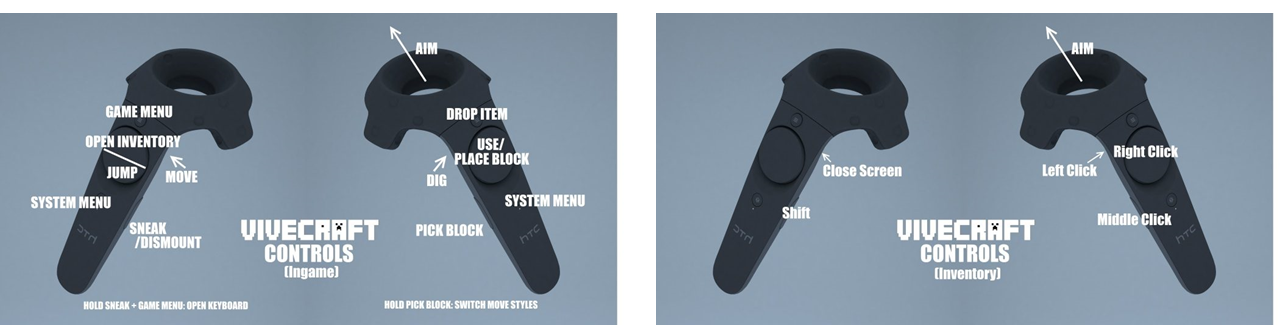
\includegraphics[width=4in]{vivecraft_controls.png}}
	\caption{Image of default button mapping for Vivecraft\cite{vivecraft_controllers}}\label{vive_craft_controls}
\end{figure}

\subsection{Interaction}
This has the same level of interaction as the original Minecraft. You can virtually interact with every part of the game. You can collect materials for the environment around you, use those materials to craft items or build things. I cool extra feature added for VR is that you can actually punch a tree with the motion controls to gather wood which is an iconic part of the original game. This game is \textbf{completely interactive}.

\subsection{Visualization}
The visuals of this game are a unique blocky cartoon-like graphics. Because of this, the resolutions seems low, but the game's graphics has a nostalgic feeling to it. 

\subsection{Social Aspects}
You can craft and explore with other players in the game which is the same as the baseline game. Additionally they added the ability to see the hand motions of players with a VR headset so you have a higher level of interaction.

\subsection{Comfort}
This game's comfort is a mixed-bag. On the one hand, this game has a very hard time keeping frame rate which leads to \textbf{major nausea}. On the other hand, this game has many options for movement which makes this game feel \textbf{mostly natural}.
\subsection{Immersion}
This game has the potential to be completely immersive. The only hold back from that is the frame rate issues. So we rate this game to be \textbf{mostly immersive}.

\section{Super Mario HD (Own Implementation)}
This was our first game that we integrated virtual reality. This game was originally just a proof of concept of how Super Mario 64 would look like in the Unity game engine. It only contains the first level of the game, but it's a good example of integration of virtual reality into a platformer. Figure \ref{SuperMarioHD_Gameplay} has a video discussing the different aspects of this game. 
  
\begin{figure}[h]
	\centering
	\centering{\hspace{0 ex}
	\includemedia[
	width=1.1\linewidth,height=0.61875\linewidth,
	activate=pageopen,
	flashvars={
		modestbranding=1 % no YT logo in control bar
		&autohide=1 % controlbar autohide
		&showinfo=0 % no title and other info before start
		&rel=0 % no related videos after end
	}
	]{}{http://www.youtube.com/v/6Pw_5EoruBg}}
		\caption{Super Mario HD Gameplay and Discussion}
		\label{SuperMarioHD_Gameplay}
\end{figure}

\subsection{Locomotion}
The movement is based on the joystick of a gamepad. It moves in the same way as Super Mario 64.
\subsection{Controls}
This game keyboard and mouse or a gamepad. We played using an Xbox One gamepad and the controls are as follows: 

\begin{itemize}
	\item The \textbf{joystick} moves the character around
	\item The \textbf{start} button brings up the menu/pauses
	\item The \textbf{select} button centers the screen
	\item The \textbf{X} and \textbf{Y} buttons Tailswipe
	\item The \textbf{A} and \textbf{B} buttons Jump
	\item The \textbf{Left or Right Bumper} does a Belly Flop while jumping
\end{itemize}
\subsection{Interaction}
In this game allows you to jump on enemies or gather coins. We would classify this as having \textbf{a little} bit of interaction which is the same as Lucky's Tale. 
\subsection{Visualization}
This the same graphics as Super Mario 64 but with higher fidelity and improved lighting and textures.
It is bright colors and cartoony. 
\subsection{Social Aspects}
This game was originally created as a demo to show how one stage of Super Mario 64 would look like in a modern engine. There was no thought or effort to integrate any social aspects into this game. 

\subsection{Comfort}
This implementation felt mostly natural. The virtual reality integration feels \textbf{somewhat natural} due to the fact that you head is tracked one-to-one but there it is hard to follow Mario when running in certain directions. It only made us feel \textbf{minor nausea}, though this may get worse with more game play time because, like Lucky's Tale, the camera follows the character. 

\subsection{Immersion}
This game is more immersive than playing on a 2D screen but overall VR made the game \textbf{a little} immersive. 

\section{FreeSpace 2 (Own Implementation)}
FreeSpace 2 is a space shooter game where you pilot a spaceship and shoot other enemy space ships. We integrated our virtual reality into the updated open source version of the game. This open source version contain graphical and engine enhancements that are needed to run on newer computers. Figure \ref{FS2_Gameplay} has a video discussing the different aspects of this game.  
 
\begin{figure}[h]
	\centering
		\centering{\hspace{0 ex}
	\includemedia[
	width=1.1\linewidth,height=0.61875\linewidth,
	activate=pageopen,
	flashvars={
		modestbranding=1 % no YT logo in control bar
		&autohide=1 % controlbar autohide
		&showinfo=0 % no title and other info before start
		&rel=0 % no related videos after end
	}]{}{http://www.youtube.com/v/n2Tv13rXDX8}}
		\caption{FreeSpace 2 Gameplay and Discussion}
		\label{FS2_Gameplay}
\end{figure}
\subsection{Locomotion}
The locomotion of the baseline game was point your mouse in the direction you wanted to go and press the acceleration key. It also utilizes significant inertia in it motions. Our VR implementation of the game moved direction of the ship to match the orientation of your head; basically replacing any mouse movement input. 

\subsection{Controls}
This game uses keyboard and mouse and is a complicated space shooter with different mappings to the different keys on the keyboard. We only really played around with a couple of the controls and they were as follows:

\begin{itemize}
	\item The \textbf{A} key Accelerates 
	\item The \textbf{T} key turned on Targeting 
	\item The \textbf{Left Mouse Button} is used to Fire  
\end{itemize} 

\subsection{Interaction}
The interactions of this game is limited to that of what you would expect from space shooter. You can move freely around the environment and shoot enemies. Generally speaking we found the game have to \textbf{a little} interaction. 


\subsection{Visualization}
Visually there are a lot of double vision issues. We had trouble with the getting the eye offsets correct set for the rendering which caused this double vision. We also had to reduce some of the extra objects in the environment to make the game play more comfortable. 
  
\subsection{Social Aspects}
There is multiplayer in the game. We have no tested this, mostly due to the fact that it would be unfair to other players that we have a control scheme that uses the HMD point the ships orientation. 
\subsection{Comfort}
This game is very uncomfortable due to the double vision issues with the HMD. This game has an \textbf{unplayable level of nausea} and the controllers are \textbf{mostly unnatural} due to the use of keyboard and mouse. 

 
\subsection{Immersion}
Due to the technical issues with the rendering, this game only has \textbf{a little immersion}. 

\section{Quake (Own Implementation)}
Quake is one of the first true 3D first person shooters. We integrated our virtual reality into an opensource version of the game call Quakespasm. This particular version of Quakespasm had integrated the Oculus Rift virtual reality system into it's game play mechanics (head oriented aiming only). We ripped out the code for the Oculus Rift and integrated the OpenVR API into the game. This enabled us to provide aiming based on the motion controllers. 

We ended up with two versions of this game. One version included the ability to walk around the gun in room scale and had movement based on where you were looking. The other version had orientation tracking only but the ability to walk around based on where the gun was pointing. Figure \ref{Quake_Gameplay} has a video discussing the different aspects of this game.  

 
\begin{figure}[h]
	\centering
	\centering{\hspace{-8 ex}
	\includemedia[
	width=1.1\linewidth,height=0.61875\linewidth,
	activate=pageopen,
	flashvars={
		modestbranding=1 % no YT logo in control bar
		&autohide=1 % controlbar autohide
		&showinfo=0 % no title and other info before start
		&rel=0 % no related videos after end
	}]{}{http://www.youtube.com/v/0DcQ6HT1N4Q}}
		\caption{Quake Gameplay and Discussion}
		\label{Quake_Gameplay}
\end{figure}

\subsection{Locomotion}
Both versions of the game uses the grip button to jump and the trackpad to move forward and backward. The main difference between the versions are what pointing was used for the forward and backward movement. Version A used the pointing of the gun for the movement direction, and version B used the pointing of your HMD for your movement direction. 

One other difference between the versions is that version A had only orientation tracking and version B allowed you to walk around in room scale relative to the gun.  

\subsection{Controls}
We mapped game controls and aiming to one of the HTC Vive's motion controller The controls are as follows: 

\begin{itemize}
	\item The \textbf{Grip} button Jumps 
	\item The \textbf{Trackpad Up} is used to move Forward 
	\item The \textbf{Trackpad Down} is used to move Backwards
	\item The \textbf{Trigger} button is used to Fire
	\item The \textbf{Menu} button is used to open Menu
	\item The controller \textbf{orientation} is used to Aim the gun's yaw, pitch, and roll.  
\end{itemize} 
\subsection{Interaction}
We did not change the interaction of the baseline game. The included interactions are the ability to shoot enemies and the ability to pick up items. We rate this to have \textbf{a little interaction}.

\subsection{Visualization}
Even though this game was based on a updated graphics build of the baseline game, it still has the feel of a 90s first person shooter. It also has a very dark palette of colors made primarily from browns and greens. 
\subsection{Social Aspects}
While quake itself has a multi-player following, our implementation of VR does not work with on-line play. This is due to the fact that packets of game information would need to be updated to add in the new player state information that was added for the VR implementation. 

\subsection{Comfort}
Version B is not very comfortable. This mainly is due to the fact that you movement is based on where you are looking. We rate this as \textbf{significantly nauseating} and only \textbf{somewhat natural}.

Version A is more comfortable than version B. This improvement is due to the movement being based on where your gun is pointing and not where your HMD is looking. We rate this as \textbf{minor nausea} and only \textbf{mostly natural}.

\subsection{Immersion}
This game is fairly immersive, with the only real drawbacks being the scale of your player is seems off and you can't independently move the gun's position. Overall we rate this game to be \textbf{mostly immersive}.



\section{Summary}
Overall we found that the best types of locomotion involved room scale movements and teleportation. This leads to more natural interactions and more comfortable experiences. We found that different visualizations did not have too much impact on our experience unless it was extremely simplistic. Immersion is improved when there is interesting game play or environments. The games with social aspects in them had a feeling of being in the same room as the other players which is something that is not experienced when playing games on a 2D display. Simplistic controls improve the naturalness of the game play and provide overall a better experience. 


\begin{thebibliography}{10}
	
	\bibitem{htc_vive} 	\textbf{HTC Vive:} http://store.steampowered.com/app/358040/HTC\_Vive/

	\bibitem{htc_vive_system_image}
	\textbf{HTC Vive System Image:} https://19818-presscdn-pagely.netdna-ssl.com/wp-content/uploads/647/cd/htc-vive-set.0.jpg

	\bibitem{juggline_htc_vive_controllers}
	\textbf{Juggling Controllers:} http://www.roadtovr.com/htc-vive-tracker-juggling-underscores-impressive-performance/
	
	\bibitem{htc_vive_system_specs}
	\textbf{HTC Vive Specs:} http://www.digitaltrends.com/virtual-reality/oculus-rift-vs-htc-vive/
	
	
	\bibitem{htc_vive_controller_buttons}
	\textbf{HTC Vive Controller:} https://koenig-media.raywenderlich.com/uploads/2016/12/ViveControllerButtons.png
	
	\bibitem{xbox_one_controller_buttons}
	\textbf{Xbox One Controller:} http://support.xbox.com/en-US/xbox-one/accessories/xbox-one-wireless-controller
		
	\bibitem{vivecraft_controllers} 
	\textbf{Vivecraft Controls:} http://www.vivecraft.org/how-to-play/
	
	\bibitem{luckys_tale_game} 
	\textbf{Lucky's Tale Game Link:} https://www.oculus.com/experiences/rift/9091\hspace{1cm} 29545868758/
	
	\bibitem{google_earth_game} 
	\textbf{Google Earth VR Software Link:} http://store.steampowered.com/app/348250/Google\_Earth\hspace{1cm} \_VR/?snr=1\_7\_15\_\_13
	
	\bibitem{destinations_game} 
	\textbf{Destinations Game Link:} http://store.steampowered.com/app\hspace{1cm} /453170/Destinations/
	
	\bibitem{climbey_game} 
	\textbf{Climbey Game Link:} http://store.steampowered.com/app/520010\hspace{1cm} /Climbey/
	
	\bibitem{thewavevr_game} 
	\textbf{TheWaveVR Game Link:} http://store.steampowered.com/app/\hspace{1cm} 453000/TheWaveVR//
	
	\bibitem{rec_room_game} 
	\textbf{Rec Room Game Link:} http://store.steampowered.com/app/\hspace{1cm} 471710/Rec\_Room/
	
	\bibitem{rickandmorty_game} 
	\textbf{Rick and Morty Game Link:} http://store.steampowered.com/app/\hspace{1cm} 469610/Rick\_and\_Morty\_Virtual\_Rickality/
	
	\bibitem{vive_craft_game} 
	\textbf{Vivecraft Game Link:}http://www.vivecraft.org/
	
	\bibitem{super_mario_hd_game} 
	\textbf{Super Mario HD Game Link:} https://www.youtube.com/watch?v=lVgvXJk7X5k
	
	\bibitem{freespace2_game} 
	\textbf{FreeSpace 2 Game Link:} https://github.ccs.neu.edu/\hspace{1cm} buildingagameengine/fs2open\_VR
	
	\bibitem{quake_game} 
	\textbf{Quake Game Link:} https://github.ccs.neu.edu/buildingagameengine\hspace{1cm} /QuakespasmOpenVR
	


	
\end{thebibliography}






\end{document}




   
